\documentclass[12pt]{report}

%%%%%%%%%%%%%%%%%%%%%%%%%%%%%%%%%%%%%%%%%%%%%%%%%%%%%%%%%%%%%%%%%%%%%%%%%%%%%

% Definitions for the title page
% Edit these to provide the correct information
% e.g. \newcommand{\reportauthor}{Timothy Kimber}

\newcommand{\reporttitle}{State Decomposition and Hierarchical Reinforcement Learning}
\newcommand{\reportauthor}{Edoardo David Santi}
\newcommand{\supervisor}{Prof. Kin K. Leung}
\newcommand{\degreetype}{Master of Engineering}

%%%%%%%%%%%%%%%%%%%%%%%%%%%%%%%%%%%%%%%%%%%%%%%%%%%%%%%%%%%%%%%%%%%%%%%%%%%%%

% load some definitions and default packages
\input{includes}

% load some macros
\input{notation}

\date{January 2021}

\begin{document}

% load title page
\begin{titlepage}
                % \newgeometry{top=25mm,bottom=25mm,left=38mm,right=32mm}
                \setlength{\parindent}{0pt}
                \setlength{\parskip}{0pt}
                % \fontfamily{phv}\selectfont

                {
                                \Large
                                \raggedright
                                Imperial College London\\[17pt]
                                Department of Electrical and Electronic Engineering\\[17pt]
                                Final Year Project Report 2021\\[17pt]
 
                }

                \rule{\columnwidth}{3pt}
                \vfill
                \centering
                  \includegraphics[width=0.7\columnwidth,height=60mm,keepaspectratio]{figures/225px-Imperial_College_London_crest.svg.png}
                \vfill
                \setlength{\tabcolsep}{0pt}

                \begin{tabular}{p{40mm}p{\dimexpr\columnwidth-40mm}}
                                Project Title: & \textbf{State-decomposition techniques for sample efficient Deep Reinforcement Learning} \\[12pt]
                                Student: & \textbf{Edoardo David Santi} \\[12pt]
                                CID: & \textbf{01373388} \\[12pt]
                                Course: & \textbf{MEng Electrical \& Electronic Engineering} \\[12pt]
                                Project Supervisor: & \textbf{Prof. Kin K. Leung} \\[12pt]
                                Second Marker: & \textbf{Dr Tania Stathaki} \\
                \end{tabular}
\end{titlepage}


% page numbering etc.
\pagenumbering{roman}
\clearpage{\pagestyle{empty}\cleardoublepage}
\setcounter{page}{1}
\pagestyle{fancy}

%%%%%%%%%%%%%%%%%%%%%%%%%%%%%%%%%%%%
%\begin{abstract}
%Your abstract
%\end{abstract}

%\cleardoublepage
%%%%%%%%%%%%%%%%%%%%%%%%%%%%%%%%%%%%
%\section*{Acknowledgments}
%Comment this out if not needed.

%\clearpage{\pagestyle{empty}\cleardoublepage}

%%%%%%%%%%%%%%%%%%%%%%%%%%%%%%%%%%%%
%--- table of contents
%\fancyhead[RE,LO]{\sffamily {Table of Contents}}
\tableofcontents 


%\clearpage{\pagestyle{empty}\cleardoublepage}
\pagenumbering{arabic}
\setcounter{page}{1}
%\fancyhead[LE,RO]{\slshape \rightmark}
%\fancyhead[LO,RE]{\slshape \leftmark}

\doublespacing
%%%%%%%%%%%%%%%%%%%%%%%%%%%%%%%%%%%%
\chapter{Project specification}

\section{Motivation}

%The online nature of this family of algorithms causes them to focus on learning optimal decisions in the most visited states at the expense of the least visited ones. $

\paragraph{}
Reinforcement learning (RL) has been a very active research area in the last few years, achieving impressive feats in a wide range of applications. Some advantages of reinforcement learning algorithms are great flexibility, the capability of solving both very low and high-level problems \cite{sutton_barto_2018} and not requiring a model of the environment in which they are used. RL has famously been used to solve games, such DeepMind's AlphaGo \cite{silver_mastering_2017}, a program that in 2016 beat the top-ranked Go player in the world. Other successful applications are in healthcare \cite{yu_reinforcement_2020}, robotics \cite{noauthor_google_nodate}, autonomous driving \cite{autonomousDriving} and natural language processing \cite{NLP}. My project supervisor Prof. K. K. Leung has also been working on applications of RL in software-defined networks (SDNs), such as for the control of the placement of services \cite{ServicePlacement} and the synchronisation of controllers in distributed SDNs \cite{SDNSynchronisation}.

\paragraph{}
Dealing with very large systems is one of the main problems encountered in the application of reinforcement learning in practical environments. RL is based on learning through interaction with the environment. As the size of the system increases, so does the complexity of the problem and it becomes increasingly difficult to learn how to interact with the environment, making the learning process longer. In practical scenarios, it might not be feasible to train an RL agent for long enough for it to be a feasible solution, as this might incur excessive costs or, in the case that the behaviour of the environment changes over time, the algorithm might not be able to learn fast enough to adapt to the changing environment.

\section{Project Definition}

\paragraph{}
The goal of this project is to develop the state-decomposition method proposed by my supervisor Prof. K. K. Leung. This aims to alleviate the problem of large state spaces of the Markov Decision Processes (MDPs) that underlay many practical environments. This new method leverages the characteristic of many control problems of being composed of many almost independent sub-problems that only seldom interact with each other. The method first identifies the sub-problems, then it trains separate RL agents for each of them. These are later combined to form a global agent that controls the whole system and takes into account their interactions. 

\paragraph{}
While the high-level methodology is defined, the specifics of the algorithms are not. This project involves conducting research on the development of the state-decomposition method and to test it and benchmark it against mainstream algorithms to determine if it achieves improved performance.

%%%%%%%%%%%%%%%%%%%%%%%%%%%%%%%%%%%%
\chapter{Background}

\section{Reinforcement learning}

\paragraph{}
"The reinforcement learning problem is meant to be a straightforward framing
of the problem of learning from interaction to achieve a goal" \cite{sutton_barto_2018}. 
\begin{figure}[H]
    \centering
    \includegraphics[width=0.6\linewidth]{figures/agent-environment-interaction.png}
    \caption{Interaction of the agent with the environment during time step $t$. Figure taken from \cite{sutton_barto_2018}}
    \label{fig:agent-env-interaction}
\end{figure}

\paragraph{}
The reinforcement learning \textit{agent} continuously interacts with the \textit{environment}. This interaction can be modelled as a sequence of time steps $t=0,1,2,3,...$\footnote{The interaction with the environment can also be modelled in continuous time, however this is outside the scope of this project.}. At each step $t$, the environment is represented by its \textit{state} $S_t \in \mathcal{S}$, where $\mathcal{S}$ is the set of all the possible states. Taking the \textit{state} as input, the agent outputs an \textit{action} $a_t \in \mathcal{A}$, where $\mathcal{A}$ is the set of all the possible actions. In the next time step $t+1$, the environment transitions to a new \textit{state}\footnote{Note that it is possible that $S_{t+1} = S_t$} $S_{t+1}$ and emits a \textit{reward} $R_{t+1} \in \mathcal{R} \subset \R$, which the agent uses as feedback information to "learn" how to interact with the environment. Each time step can then be represented by the $\langle S_t,A_t,R_{t+1},S_{t+1} \rangle$ tuple.

\paragraph{}
The agent implements a mapping from the possible states to the probabilities of choosing the different actions. This mapping is called \textit{policy} and at time step $t$, it adopts symbol $\pi_t$. The probability of choosing action $A_t=a$ given the current state $S_t=s$ is denoted by $\pi_t(a|s)$. The goal of reinforcement learning is to learn the optimal policy, which is the policy that maximises the rewards, through repeated interaction with the environment. In general, we aim to maximise a function of the rewards at all time steps rather than the immediate reward, so the optimal policy doesn't necessarily maximise immediate rewards. The simplest case is to maximise  
\begin{equation}
    G_t =R_{t+1} + R_{t+2} + R_{t+3} + ... + R_T
\end{equation}
where $T$ is a final time step. This approach can be used when the agent-environment interaction has an end, in which case a sequence of interactions from the initial time to time $T$ can be called an \textit{episode}. In other cases, the interactions can continue indefinitely, thus this reward function is not feasible as $T=\infty$ and $G_t$ could be infinite. To fix this, we apply a \textit{discount rate} $\gamma$, with  $|\gamma|<1$, to future rewards:
\begin{equation}
    G_t=R_{t+1} + \gamma R_{t+2} + \gamma^2 R_{t+3} + ... = 
    \sum_{k=0}^\infty \gamma^{k} R_{t+k+1}
\end{equation}
This allows $G_t$ to have a finite value in continuing tasks, which are those tasks that don't have finite time episodes.

\paragraph{}
In general, the dynamics of the environment could depend on the whole history of states, rewards and actions over an episode. However, we aim to have an agent which can choose the optimal action at each time step based only on the current state. Thus the knowledge of the current state and action should give the maximum possible amount of information about the dynamics of the environment. This is true if knowledge of the history of states, rewards and actions in the previous time steps does not provide any additional information about the dynamics of the environment than knowing the current state. States that follow this property are said to follow the \textit{Markov property}. More formally, if the states follow this property
\begin{align}
    Pr\{R_{t+1}=r, S_{t+1}=s'|S_0,A_0,R_1,...,S_{t-1},A_{t-1},R_t,S_t,A_t\} \\
    = Pr\{R_{t+1}=r, S_{t+1}=s'|S_t,A_t\} \\
    = p(s',r|s,a)
\end{align}
This is the equation that governs Markov Decision Processes (MDPs) and hence a reinforcement learning task formulated with states that follow the Markov property is an MDP. 
\begin{figure}[H]
    \centering
    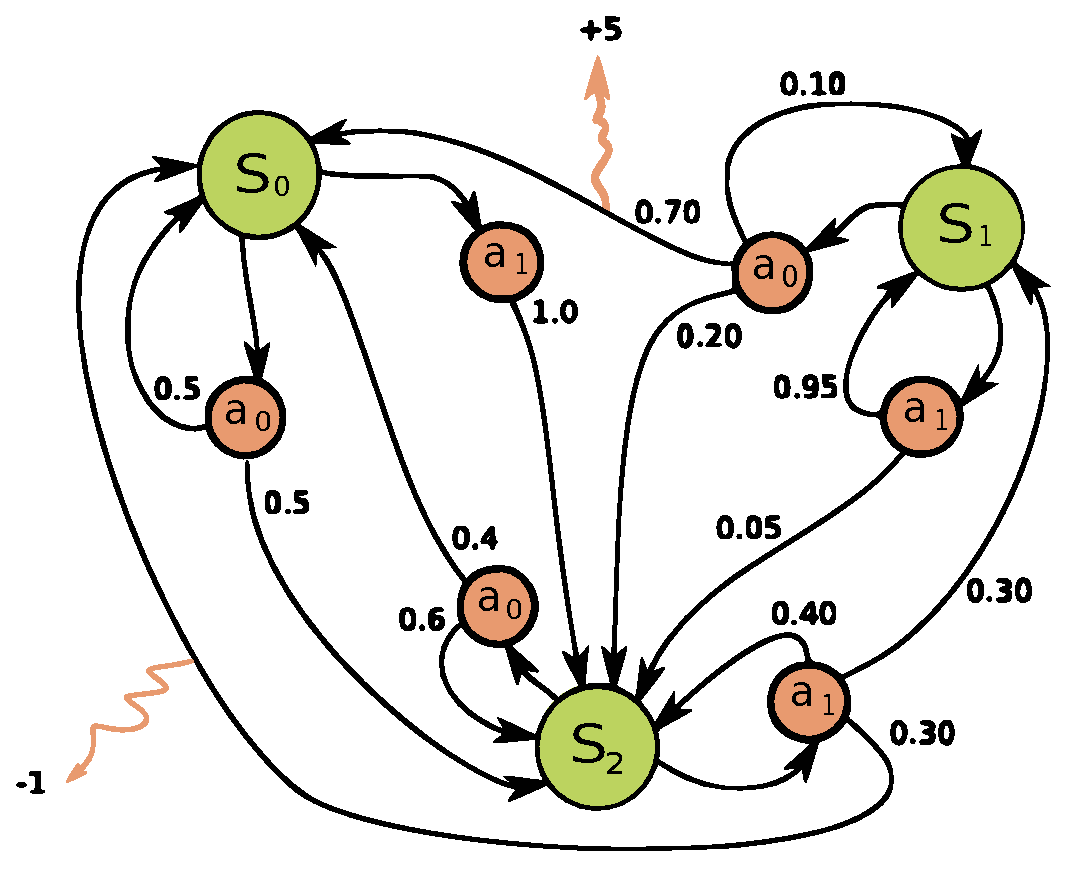
\includegraphics[width=0.5\linewidth]{figures/MDP.eps}
    \caption{Graph representation of a Markov Decision Process. Note the rewards (zigzag arrows) that are released in certain transitions. \cite{noauthor_markov_2021}}
    \label{fig:MDP}
\end{figure}

\paragraph{}
Most reinforcement learning algorithms involve the estimation of the \textit{value functions}, which are functions of states or state-action pairs. A value function represents how good it is to be in a certain state or to perform a certain action in a certain state, in terms of the expected return $G_t$ and given that we are following a certain policy. The action-value function is defined as
\begin{equation}
    q_{\pi}(s,a)=\E_\pi[G_t|S_t=s,A_t=a]=\E_\pi\left[\sum_{k=0}^\infty \gamma^{k} R_{t+k+1}|S_t=s,A_t=a\right]
\end{equation}

Similarly, the state-value function is given by
\begin{align}
    v_{\pi}(s)=\E_\pi[G_t|S_t=s]\\
    =\E_\pi\left[\sum_{k=0}^\infty \gamma^{k} R_{t+k+1}|S_t=s\right]\\
    =\sum_a \pi(a|s) \E_\pi\left[\sum_{k=0}^\infty \gamma^{k} R_{t+k+1}|S_t=s,A_t=a\right]\\
    =\sum_a \pi(a|s) q_{\pi}(s,a)
\end{align}

It is useful to specify the value functions in recursive format, known as the Bellman equations. This gives:
\begin{align}
    v_{\pi}(s)=\E_\pi[G_t|S_t=s]\\
    =\E_\pi[R_{t+1}+\gamma G_{t+1}|S_t=s]\\
    =\sum_a \pi(a|s) \sum_{s',r}p(s',r|s,a)[r+v_\pi(s')]%, \,\,\, \forall s\in\mathcal{S}
\end{align}
and
\begin{align}
    q_{\pi}(s,a)=\E_\pi[G_t|S_t=s,A_t=a]\\
    =\E_\pi[R_{t+1}+\gamma G_{t+1}|S_t=s,A_t=a]\\
    =\sum_{s',r}p(s',r|s,a)[r+v_\pi(s')]%, \,\,\, \forall \in\mathcal{S}
\end{align}

\paragraph{}
For finite MDPs it can be proved that there always exists an \textit{optimal policy} that maximises the state-values of all states the action-values of all state-action pairs, giving the optimal state-values $v_*(s)$ and $q_*(s,a)$:
\begin{align}
    v_*(s)=\max_\pi v_\pi(s), \,\,\, \forall s \in \mathcal{S} \\
    q_*(s,a)=\max_\pi q_\pi(s,a), \,\,\, \forall s \in \mathcal{S}, \,\,\, \forall a \in \mathcal{A}
\end{align}

\paragraph{}
Given full knowledge of the dynamics of the system\footnote{The probabilities of state-transitions and rewards given the current state-action pair} and a fixed policy, we are able to evaluate the optimal state-values and action-values using methods based on dynamic programming \cite{bellman_dynamic_1966}. One such method called \textit{iterative policy evaluation}, which adopts the update step based on the Bellman equations given below, can be shown to converge to the state-values:

\begin{equation}
    v_{k+1}(s)=\sum_{a\in\mathcal{A}}\pi(a|s)\left[R(s,a)+\gamma\sum_{s'\in\mathcal{S}}P(s,s',a)v_k(s')\right]
\end{equation}

\textit{Policy iteration} is one possible method of evaluating the state values when the optimal policy is not given, which alternates steps of policy evaluation and updates of the policy. The policy is updated so that in every state the greedy action, meaning the one with the highest action-value, is always picked. This process of solving the MDP when given the model of the environment is known as \textit{planning}. 

\paragraph{}
However, in many applications the model of the environment is unknown. Given a certain policy, it is possible in this case to approximate the state and action values by sampling the interaction with the environment. Monte Carlo methods interact with the environment by following the given policy and approximate each state-value using the returns obtained in each episode after the first or each visit to the state. The update that occurs every time the state occurs for the first time in the episode  (or every time, depending on the version of the algorithm) is
\begin{equation}
    V(S_t) \leftarrow V(S_t)+\alpha[G_t - V(S_t)]
\end{equation}
The disadvantage is that state-values cannot be updated until the end of an episode. Temporal Differences methods are another class of methods that solve this problem. Instead of relying on returns ($G_t$), they approximate them as the sum of the reward and the discounted state-value of the next visited state. The simplest TD algorithm's update step is given by
\begin{equation}
    V(S_t) \leftarrow V(S_t)+\alpha(R_{t+1} + \gamma V(S_{t+1})-V(S_t))
\end{equation}

\paragraph{}
There are many applications of reinforcement learning in which state-space and action-spaces are continuous. In that case, the MDP is not finite as there is an infinite number of possible states and actions. This will not be discussed as it is outside of the scope of this project, which only deals with discrete state and action spaces.


\section{Q-learning and Deep Q-learning}

\paragraph{}
Many RL algorithms deal with the problem of solving an MDP without being given the optimal policy and the dynamics of the system. Q-learning \cite{watkins_1989} is one of the most noteworthy among these. It is based on Temporal Differences learning as the action-value updates follow a very similar formula. The basic value update in Q-learning is given by:
\begin{equation}
    Q(S_t, A_t) \leftarrow Q(S_t, A_t) + \alpha[R_{t+1}+\gamma \max_a Q(S_{t+1},a) - Q(S_t,a)]
\end{equation}
Differently from the previously described TD algorithm, this operates on action-values instead of state-values. In Q-learning, the value update is done using the term $\max_a Q(S_{t+1},a)$, which is the action-value of the greedy-action in the next visited state. This is not necessarily the action taken in the following step when visiting $S_{t+1}$, thus this an \textit{off-policy} algorithm.

\paragraph{}
Differently from the Temporal Differences algorithms that aim at evaluating a fixed policy, Q-learning also deals with the control problem of choosing the policy. Q-learning is normally programmed so that its current policy is based on its current action-value estimates. An example is the $\epsilon$-greedy policy, in which at each time step, the greedy action is picked with probability $1-\epsilon$ and a random action is picked with probability $\epsilon$.

\paragraph{}
This algorithm is only defined for discrete environments and it is proven to converge to the optimal action-values with a probability of 1, as long as all the states and actions are visited multiple times \cite{watkins_q-learning_1992}. This requirement might not be feasible when the number of states is very large and it is impossible when the number of states is infinite such as when the MDP's state-space is continuous. Using a learned Q-function approximator instead of simply storing the action-values in tabular form can solve this issue, as it is possible to learn a mapping function that generalises over the whole state-space without having to visit all the possible states.

\paragraph{}
Deep Q-Learning (DQN) \cite{mnih_human-level_2015} implements the Q-function approximator using a deep neural network. This was demonstrated to achieve state-of-the-art performance in learning to play Atari games directly from the pixel data \cite{dqn}. DQN takes advantage of the ability of deep learning to learn from high-dimensional data representations to be able to directly feed large state-spaces into the agent. Deep neural networks rely on the assumption that they are fed independent samples, however in reinforcement learning the samples are correlated as they are generated by a temporal sequence. An \textit{experience replay} is used to solve this. The transition samples are saved in memory and a random batch is selected to train the neural network at each time-step, thus removing correlations due to temporal proximity of the samples. This also allows the update to be based on a batch, rather than a single sample, which improves the sample efficiency\footnote{How efficiently the samples are used by the algorithm to learn. A more sample efficient algorithm requires fewer interactions with the environment to learn an optimal policy.}.

\paragraph{}
One issue of the Q-learning algorithm is that using the maximum action value of the next visited state in the update step results in a positive bias in the estimation of the action values, which can lead to poor performance in some stochastic environments. Double Q-learning \cite{wiskunde_doubleq-learning_nodate} deals with this problem by splitting the samples randomly between two separate sets of action value estimates and by updating the values of each set of estimates using the values of the other, which can be proven to remove the positive bias\footnote{It actually introduces a small negative bias, thus tending to underestimate the action values.}. The same problem persists in deep Q-learning and a similar solution has been devised in Double Deep Q-Learning \cite{van_hasselt_deep_2015}. Another version of DQN that achieved improved performance in typical benchmarks such as playing Atari games is Dueling DQN \cite{wang_dueling_nodate}, which operates on the concept of expressing action values as a sum of state values and advantages: $\mathcal{Q}_\pi(s,a)=\mathcal{V}_\pi(s)+\mathcal{A}_\pi(s,a)$.

\paragraph{}
While the original Q-learning algorithm can only be applied to systems with discrete state and action spaces, other algorithms based on Q-learning have been proposed to deal with continuous state and action spaces, such as Wire Fitted Neural Network Q-learning \cite{goos_q-learning_1999}.


\section{Problem of large state-spaces}

\paragraph{}
Very large systems correspond to MDPs with a very large number of states, which can be difficult to solve using reinforcement learning algorithms. The number of possible state-transitions is the square of the number of states, thus the complexity of controlling a system grows very quickly as the size of a system increases, and learning an optimal policy becomes very difficult and often infeasible.

\paragraph{}
Various approaches have been used to solve this issue. One general approach is to learn representations of the states to improve generalisation to unseen states or to decrease the dimensionality of the states by compression. DQN \cite{dqn} exploits the ability of deep learning to learn from high-dimensional data and to generalise to solve this issue, though this is often not sufficient. \cite{stateActionEmbeddings} jointly learns state and action embeddings to improve generalisation. In World Models \cite{worldModels}, a compressed latent representation of the states is explicity learned by an autoencoder, which is then fed into the reinforcement learning model instead of the original states. Other methods rely on state aggregation \cite{stateAggregation}, in which states with similar state-transition probabilities and rewards are grouped to form a higher-level state. This technique can also be applied to hierarchical reinforcement learning to define the states of the global learner \cite{aggregationHierarchical}. 

\paragraph{}
Hierarchical reinforcement learning \cite{barto_recent_2003} is another approach that reduces the impact of large state spaces. Hierarchical RL provides temporal abstraction by subdividing the main task into sub-tasks. For example, the task of commuting to work can be subdivided into sub-tasks such as opening a door, turning right, walking to the tube station, etc. The agent is composed of hierarchies of sub-agents in which each sub-agent is fed a compressed or reduced state space in input and outputs high-level actions to its "children" sub-agents that perform the lower-level actions required to complete the received higher-level action. Examples of hierarchical reinforcement learning algorithms are based on MAXQ value decomposition \cite{dietterich_hierarchical_1999}, Options \cite{sutton_between_1999} and Hierarchies of Machines (HAM) \cite{parr_reinforcement_nodate}. 

\paragraph{}
Model-based reinforcement learning \cite{moerland_model-based_2020} has been receiving increasing attention lately. This class of algorithms is at the intersection of planning algorithms and model-free reinforcement learning as it approximates the model of the environment during the learning process, which can be used to more efficiently learn from new samples. Dyna \cite{sutton_dyna_1991} learns a model of the environment and uses it to simulate samples for Q-learning other than those obtained by actual interaction with the environment. AlphaZero \cite{silver_mastering_2017}, which achieved state-of-the-art performance in playing Chess, leverages full knowledge of the model\footnote{The model is given at the start rather than learnt.} to perform a Monte-Carlo tree search for every step in the real-world environment. \cite{worldModels} trains an RNN model that predicts the following state at each-time step. Though this class of algorithms does not explicitly tackle the problem of large state-spaces, the improvements in sample efficiency can still solve the issue by allowing to train a model with fewer interactions with the environment. 

\section{State-Decomposition method}

\paragraph{}
The main topic of this project is the development of the state-decomposition method. This is suited to control problems of environments that are composed of many sub-problems that only seldom interact with each other. Separate RL agents can be trained for these separate sub-problems independently, thus treating them as separate problems. The separate agents are then combined at a later stage to take into account the interactions between the sub-problems. 

\paragraph{}
The first step of the process is to identify the subsystems as groups of states. This is done by examining the state-transition probability matrix. Given a finite MDP, this is defined as the matrix where each entry $P_{ij}$ is the probability of transitioning from state $S_t=i$ to the next state $S_{t+1}=j$:

\begin{equation}
    \begin{bmatrix}
    P(S_{t+1}=s_0|S_{t}=s_0) & P(S_{t+1}=s_1|S_{t}=s_0) & ... & P(S_{t+1}=s_n|S_{t}=s_0) \\
    P(S_{t+1}=s_0|S_{t}=s_1) & P(S_{t+1}=s_1|S_{t}=s_1) & ... & P(S_{t+1}=s_n|S_{t}=s_1) \\
    ... & ... & ... & ... \\
    P(S_{t+1}=s_0|S_{t}=s_n) & P(S_{t+1}=s_1|S_{t}=s_n) & ... & P(S_{t+1}=s_n|S_{t}=s_n) \\
    \end{bmatrix}
\end{equation}

where $n$ is the number of states in $\mathcal{S}$. 

\begin{figure}[H]
\centering

\begin{tikzpicture}[font=\sffamily]

        % Setup the style for the states
        \tikzset{node style/.style={state, 
                                    minimum width=1cm,
                                    line width=0.5mm,
                                    fill=gray!20!white}}

        % Draw the states
        \node[node style] at (0, 0) (0) {0};
        \node[node style] at (3, 0) (1) {1};
        \node[node style] at (0, -3) (2) {2};
        \node[node style] at (3, -3) (3) {3};

        % Connect the states with arrows
        \draw[every loop,
              auto=right,
              line width=0.5mm,
              >=latex,
              draw=orange,
              fill=orange]
            (2)     edge[bend right=20]            node {} (0)
            (2)     edge[bend right=20, auto=left] node {} (1)
            (2)     edge[bend right=20, auto=left] node {} (3)
            (2)     edge[loop left=20, auto=left] node {} (2)
            (1)     edge[bend right=20]            node {} (2)
            (1)     edge[bend right=20, auto=left] node {} (0)
            (1)     edge[loop right=20, auto=left] node {} (1)
            (1)     edge[bend right=20, auto=left] node {} (3)
            (0) edge[bend right=20]            node {} (1)
            (0)     edge[bend right=20, auto=left] node {} (3)
            (0) edge[bend right=20, auto=left] node {} (2)
            (0)     edge[loop left=20, auto=left] node {} (0)
            (3) edge[bend right=20]            node {} (1)
            (3)     edge[bend right=20, auto=left] node {} (0)
            (3) edge[bend right=20, auto=left] node {} (2)
            (3)     edge[loop right=20, auto=left] node {} (3);;
\end{tikzpicture}
\begin{tikzpicture}
    \draw[->,line width=2pt]
  ([xshift=-5pt,yshift=-60pt]pic cs:starta) -- node[above,align=center] {\strut Apply \\ threshold \strut}
  ([xshift=15pt,yshift=-60pt]{{pic cs:enda}|-{pic cs:starta}});
\end{tikzpicture}
\begin{tikzpicture}[font=\sffamily]

        % Setup the style for the states
        \tikzset{node style/.style={state, 
                                    minimum width=1cm,
                                    line width=0.5mm,
                                    fill=gray!20!white}}

        % Draw the states
        \node[node style] at (0, 0) (0) {0};
        \node[node style] at (3, 0) (1) {1};
        \node[node style] at (0, -3) (2) {2};
        \node[node style] at (3, -3) (3) {3};

        % Connect the states with arrows
        \draw[every loop,
              auto=right,
              line width=0.5mm,
              >=latex,
              draw=orange,
              fill=orange]
            (2)     edge[bend right=20, auto=left] node {} (3)
            (2)     edge[loop left=20, auto=left] node {} (2)
            (1)     edge[bend right=20, auto=left] node {} (0)
            (1)     edge[loop right=20, auto=left] node {} (1)
            (0) edge[bend right=20]            node {} (1)
            (0)     edge[loop left=20, auto=left] node {} (0)
            (3) edge[bend right=20, auto=left] node {} (2)
            (3)     edge[loop right=20, auto=left] node {} (3);;
\end{tikzpicture}

\caption{Applying a threshold to the state transition matrix and normalising the probabilities can cause the MDP to separate into separate MDPs as it reduces the number of possible transitions.}

\label{fig:OneMDPtoManyMDPs}

\end{figure}

\paragraph{}
The state-decomposition method is based on the fact that some state-transition probabilities are negligible compared to others and could be regarded as 0 to obtain a sparse version of the state-transition matrix. Specifically, every element smaller than a threshold $\epsilon$ can be set to 0. The probabilities of the matrix can then be normalised so that each row of the matrix has a sum of 1. This step is unnecessary and can be skipped in the implementation; however, it is necessary to obtain a valid MDP from the state-transition matrix after applying the threshold. Following this procedure, the MDP could be formed by multiple independent MDPs with smaller state-spaces, as shown in Figure-\ref{fig:OneMDPtoManyMDPs}. In this case, by reordering the states it is possible to express the state-transition matrix as a block matrix in the form:

\begin{equation}
    \begin{bmatrix}       
    \fbox{$B_1$} & 0 & ... & 0  \\
     0 & \fbox{$B_2$} & ... & 0 \\
     ... & ... & ... & ... \\
     0 & 0 & ... & \fbox{$B_n$} \\
   \end{bmatrix}
\end{equation} 

where the matrices $B_1, B_2, ..., B_n$ are the state-transition matrices of the newly formed separate MDPs.

\paragraph{}
Once the states of the original MDP have been separated into multiple sub-spaces, it is possible to proceed with training the RL agent. In the first stage of training, for each of these sub-spaces, we train a separate DQN agent. To do so, we consider for each sub-space's agent only those state transitions that start and end within the same sub-space. Once the sub-spaces' agents converge\footnote{Or earlier. The time when we should do this is to be researched in this project.}, these should be combined to form a global agent that also takes into account transitions between the different sub-spaces. This is done by feeding the action values of the sub-spaces' agents, which are the outputs of their neural networks, as inputs of another neural network, as in Figure-\ref{fig:join_nets}. This forms a bigger neural network which is the Q-function approximator of a new global DQN agent, which is then trained using all possible transitions. This will be referred to as the second stage of training.

\begin{figure}[H]
    \centering
    \includegraphics[width=0.5\linewidth]{figures/join_networks}
    \caption{The NNs of the decomposed states' agents are merged as input of another NN to form a new bigger NN.}
    \label{fig:join_nets}
\end{figure}

\paragraph{}
This method operates on the assumption that it would require fewer samples to achieve convergence for RL agents operating on many smaller MDPs than on one single MDP having as the number of states the sum of the number of states of the smaller MDPs. This is because the number of possible transitions in an MDP is the square of the number of states, so by dividing the system into separate independent sub-problems we reduce the complexity of the control problem\footnote{By decreasing the number of possible transitions, as \(\sum_{i=0}^n x_i^2 \leq (\sum_{i=0}^n x_i)^2\)}. By then combining the neural networks as previously explained, we take into account interactions between the sub-problems, allowing us to achieve the optimal policy for the original MDP. For this method to be successful, it is assumed that the weights of the neural networks of the sub-spaces' agents are not far from the values they take once the global agent converges in the final stage of training. This is equivalent to saying that the first stage of training provides a very good initialisation of the weights of the network used in the second stage. Although we use DQN agents, this method could be generalised to any agents that use a function approximator to evaluate the action-values given in input the states. This method however wouldn't be as useful if no approximator is being used, and the action-values are simply stored in a table, such as in the original Q-learning algorithm. In this case, applying the state-decomposition would simply ignore the transitions between different sub-spaces without changing the structure of the agent at all in the first stage of training.


%%%%%%%%%%%%%%%%%%%%%%%%%%%%%%%%%%%%
\chapter{Implementation Plan}

\paragraph{}
The state-decomposition method is going to be implemented and tested in multiple varieties to assess the effect it has when applied to reinforcement learning algorithms. 

\section{Tools}

\paragraph{Python}
The programming language chosen for this project is Python. This is motivated by Python being a high-level language that allows writing compact, readable code and by the widespread availability of resources and packages for it (such as the OpenAI Gym toolkit previously described). Additionally, Python can be run on Colab notebooks.

\paragraph{Google Colaboratory}
Google Colab is a platform from Google which is widely used for machine learning research and prototyping of new models. Colab combines a notebook platform that many Python developers are familiar with and the high-performance of cloud computing. The user can choose to run a program using CPUs, GPUs, or TPUs\footnote{Tensor Processing Unit: a custom hardware accelerator developed by Google to accelerate the linear algebra operations that occur in machine learning. \cite{noauthor_cloud_nodate}}. Examples of the available GPUs are Nvidia K80 and NVidia P100D. The disadvantage of Colab compared to cloud computing platforms such as Google Cloud and Amazon AWS is that the user is not guaranteed full access to the hardware accelerators (such as GPUs) and thus the performance can vary. The session length is also limited to 12 hours. These problems are mitigated by purchasing a "Pro" license for the price of \$10 per month, which prioritises access to GPUs and increases the maximum session length to 24 hours. The level of performance offered by Colab Pro is enough for this project. The main advantage is an easy to use platform thanks to its notebook format, rather than the less user-friendly access via SSH in the Terminal required by other cloud-computing platforms. 

\paragraph{Keras}
It was decided to implement the deep-learning models using the deep-learning API Keras \cite{keras}. This is a high-level interface that uses Tensorflow \cite{noauthor_tensorflow_nodate} for its backend. Keras allows to code deep-learning models in a very readable and compact way. Having Tensorflow as its backend, it can run on CPUs, GPUs, and TPUs, taking advantage of the high-performance hardware offered by Google Colab.

\paragraph{OpenAI Gym}
As this project deals with the development and evaluation of a new method for reinforcement learning algorithms, it was decided to apply it in a "toy environment" that would simplify experimentation. OpenAI offers an open-source Python toolkit called "OpenAI Gym" \cite{openai_gym_nodate}, which is currently the most commonly used toolkit to benchmark reinforcement learning algorithms. This toolkit offers a variety of different environments, ranging from classical control problems such as "CartPole-v0" \cite{noauthor_openai_nodate}, to more complicated environments such as playing Atari games using the pixel data as sensory input or solving robotic manipulation problems. The "OpenAI Gym" offers environments with a wide range of complexities and all combinations of discrete and continuous state and action spaces.

\begin{figure}[H]
    \centering
    \includegraphics[width = 0.5\linewidth]{figures/cartpole.PNG}
    \caption{The CartPole-v1 environment is one of the most well-known environments of the OpenAI Gym library in which the goal is to balance the cartpole while keeping it within the boundaries of the screen by applying a leftwards or a rightwards force at each time-step. Screenshot of \cite{noauthor_openai_nodate}}
    \label{fig:cartpole}
\end{figure}

\section[Obtaining the state trans. matrix]{Obtaining the state transition matrix}

\paragraph{}
The first step in the state-decomposition method is to obtain the state-transition matrix. Since we are testing the algorithm in software simulations, the state-transition matrix can be easily obtained from the source code of the environments and it can be considered as given. This is usually not the case, so at a later stage we shall test methods to approximate the state-transition matrix. This can be done by interacting with the environment and sampling the $\langle S,A,R,S' \rangle$ tuples that are generated. Since the state-transition probabilities are dependent on the action, the state-transition matrix is dependent on the chosen policy. As we are conducting this before the training and we have no information about the optimal policy, we choose to use the most general possible policy to obtain the state-transition table, that is, the actions are all chosen with equal probability independently of the current state. The number of iterations required to construct the state-transition matrix is dependant on the number of states, actions, the probability of visiting each different state and the required level of accuracy of the state-transition matrix estimate. 


\section[Decomposing state trans. matrix]{Decomposing the state transition matrix}

\paragraph{}
The decomposition into sub-spaces of states given the state-transition table is done using Algorithm-\ref{algo:decompose}. The Python code for this is given in the Appendix.

\begin{algorithm}[H]
\singlespacing
\SetAlgoLined

\SetKwInOut{In}{stateTransMatrix}
\SetKwInOut{Output}{subspaces}

\SetKwData{STMat}{stateTransMatrix}
\SetKwData{Out}{subspaces}

\SetKwData{Subs}{subspaces}

\SetKwData{Thre}{$\tau$}

\In{input 2D array representing the state-transition matrix}
\Output{output data structure representing the decomposed sub-spaces}

\BlankLine
\Subs = initialise as one subspace for each group;

 \For{$i \leftarrow 0$ \KwTo height(\STMat)-1}{
 \For{$j \leftarrow 0$ \KwTo width(\STMat)-1}{
  \lIf{\STMat[$i$][$j$] $>$ \Thre}{joinSubspacesContaining($i$, $j$)}
 }
 }
 
 
 \caption{State-decomposition algorithm.}
 \label{algo:decompose}
\end{algorithm}

\paragraph{}
Sometimes we know the number of sub-spaces that the original MDP should be decomposed into. For example, we might know the characteristics of the system and the number of subsystems it can be considered to have, such as how many sub-networks compose a certain communication network. In such case, the function that returns the decomposed sub-spaces can be run repeatedly while updating the threshold value $\epsilon$ at each iteration using binary search, until the MDP is decomposed in the correct number of sub-spaces. This is given in Algorithm-\ref{algo:threshold} and the Python code is in the Appendix. 

\begin{algorithm}[H]
\singlespacing
\SetAlgoLined

\SetKwInOut{In}{stateTransMatrix}
\SetKwInOut{Output}{subspaces}
\SetKwInOut{des}{nSubspacesDesired}

\SetKwData{STMat}{stateTransMatrix}
\SetKwData{Out}{subspaces}

\SetKwFunction{SD}{stateDecomposition}
\SetKwFunction{NSubs}{nSubspaces}

\SetKwData{N}{nSubspacesDesired}
\SetKwData{MaxIt}{maxIterations}
\SetKwData{Fact}{changeFactor}
\SetKwData{Thre}{$\tau$}
\SetKwData{UB}{upperBound}
\SetKwData{LB}{lowerBound}

\In{input 2D array representing the state-transition matrix}
\des{input integer representing the number of subspaces to decompose into} 
\Output{output data structure representing the decomposed subspaces}

\MaxIt $\leftarrow 50$\;
\Fact $\leftarrow 10$\;
\Thre $\leftarrow 1.0$\;
\BlankLine
\UB $\leftarrow$ NONE\;
\LB $\leftarrow$ NONE\;
\BlankLine
 \For{$i \leftarrow 1$ \KwTo \MaxIt}{
  \If{\UB and \LB are defined}{\Thre $\leftarrow (\UB + \LB) / 2$\;}
   \lIf{only \UB is defined}{\Thre $\leftarrow \UB / \Fact$}
   \lIf{only \LB is defined}{\Thre $\leftarrow \LB * \Fact$}
   \BlankLine
   \Out $\leftarrow$ \SD(\STMat, \Thre)\;
   \BlankLine
   \lIf{$\NSubs(\Out) == \N - 1$}{break}
   \lIf{$\NSubs(\Out) < \N - 1$}{\LB = \Thre}
   \lIf{$\NSubs(\Out) > \N - 1$}{\UB = \Thre}
 }
 
 
 \caption{State-decomposition into given number of subspaces}
 \label{algo:threshold}
\end{algorithm}

\section{The need for a suitable environment} \label{sec:TaxiTraps}

\paragraph{}
The state-transition matrices and their decomposed versions were obtained for 4 different OpenAI Gym environments: "Cartpole-v1"\footnote{This environment has continuous states which are discretised using a linear quantiser to apply the decomposition algorithm.}, "FrozenLake8x8-v0", "CliffWalking-v0" and "Taxi-v3". The state-decomposition algorithm is aimed at environments whose state-spaces decompose into similarly sized sub-spaces, as this is the case in which the method would be potentially very effective. If one of the state-spaces is much greater than the others and similar in size to the original state-space, the reduction in complexity of the training in the first stage would not compensate for the more complex multi-stage nature of the state-decomposition method. Having sub-spaces that are too small (in the extreme case having just one state) limits the amount of learning that can be achieved in the first stage of training, simply delaying this to the second stage. The MDPs of "Cartpole-v1", "FrozenLake8x8-v0", "CliffWalking-v0", always decompose into one big sub-space and sub-spaces formed by only one state. This occurs because these environments are not formed of almost independent sub-problems that rarely interact with each other. 

\paragraph{}
The "Taxi-v3" environment, shown on the left in Figure-\ref{fig:taxi} is a more suitable candidate. The environment presents:
\begin{itemize}
    \item 500 discrete spaces, corresponding to 25 taxi positions in the 5x5 grid, 4 possible destinations, and 5 possible passenger positions (1 of which is inside the taxi).
    \item 6 discrete actions: 4 moves (up, down, left, right), pick-up passenger, and drop-off passenger.
    \item Rewards: +20 for a successful drop-off, -1 at each time step (also when hitting a wall), and -10 for illegal pick-up and drop-off actions.
\end{itemize}

An episode terminates when the passenger is successfully dropped off or after 200 time-steps. Applying the state-decomposition to this environment can form 4 equally sized sub-spaces even with a threshold of 0, meaning that these are 4 completely independent sub-spaces that can be treated as independent Markov Decision Processes. These 4 sub-spaces correspond to the 4 possible destinations of the passenger, which never change during a single episode. Thus, this a more specific and easier problem than the one we are trying to solve, where the subsystems, though rarely, do interact with each other. Thus, this environment is not suitable for testing the state-decomposition algorithm as good performance of the algorithm in this simpler environment does not imply good performance in the more general scenario. 

\paragraph{}
These problems in finding a suitable environment suggest that the best solution would be to create a custom environment with the characteristics that would allow better testing of the method. The "Taxi-v3" environment is composed of 4 independent MDPs. Modifying its transition-probabilities so that interaction between them is possible\footnote{Making transition-probabilities between spaces of different subsystems non-zero.}, would make this environment suitable for testing the decomposition algorithm. For this purpose, I propose a modified version called "TaxiTraps", with added "traps" located on the edges of certain squares. These activate with a low probability $p_{trap}$ when the Taxi moves over them. If a trap does not activate, the taxi simply moves over it as in the original "Taxi-v3" environment. When the trap does activate, the behaviour of the environment is modified in two ways:

\begin{enumerate}
    \item The destination of the Taxi changes. This makes it possible for the destination of a passenger to change during an episode, thus providing the transitions between different sub-spaces that exist in the general problem that the state-decomposition method is aimed at.
    
    \item A highly negative reward is released. This was added to ensure that the optimal policy in the "TaxiTraps" environment is different than in the original Taxi environment. Since in the first step of the state-decomposition method the transitions between different state sub-spaces are ignored, the agents are trained in an environment equivalent to the original "Taxi-v3". If the optimal policy is the same in "Taxi-v3" and "TaxiTraps", the optimal policy would not change between the first and second training stage of training, which is unlikely to happen in a general scenario. Thus, ensuring that the optimal policy changes between training stages is required for the results of testing to generalise to other environments.  
\end{enumerate}

%Is the fact that we are discouraging the Taxi to go over the traps a problem as in the final policy we are kind of ignoring transitions because we actively avoid them?

\begin{figure}[H]
\centering
    \resizebox{\linewidth}{!}{
    \subfloat["Taxi"]{
        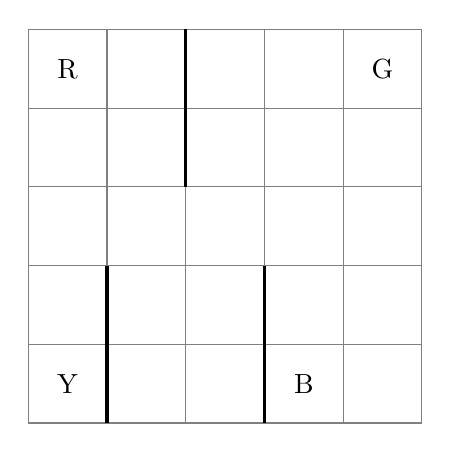
\begin{tikzpicture}
            \draw[step=1cm,color=gray] (0,0) grid (5,5);
            \node at (0.5,4.5) {R};
            \node at (4.5,4.5) {G};
            \node at (0.5,0.5) {Y};
            \node at (3.5,0.5) {B};
            \draw[very thick] (2,5) -- (2,3);
            \draw[very thick] (1,2) -- (1,0);
            \draw[very thick] (3,2) -- (3,0);
        \end{tikzpicture}}
    \qquad
    \subfloat["TaxiTraps"]{
        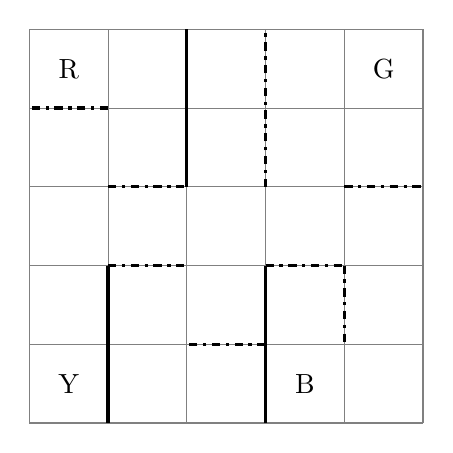
\begin{tikzpicture}
            \draw[step=1cm,color=gray] (0,0) grid (5,5);
            \node at (0.5,4.5) {R};
            \node at (4.5,4.5) {G};
            \node at (0.5,0.5) {Y};
            \node at (3.5,0.5) {B};
            \draw[very thick] (2,5) -- (2,3);
            \draw[very thick] (1,2) -- (1,0);
            \draw[very thick] (3,2) -- (3,0);
            \draw[very thick, dash dot] (1,4) -- (0,4);
            \draw[very thick, dash dot] (1,3) -- (2,3);
            \draw[very thick, dash dot] (3,1) -- (2,1);
            \draw[very thick, dash dot] (1,2) -- (2,2);
            \draw[very thick, dash dot] (3,2) -- (4,2);
            \draw[very thick, dash dot] (4,3) -- (5,3);
            \draw[very thick, dash dot] (3,3) -- (3,5);
            \draw[very thick, dash dot] (4,2) -- (4,1);
        \end{tikzpicture}}
    \qquad
    \subfloat["Taxi2"]{
        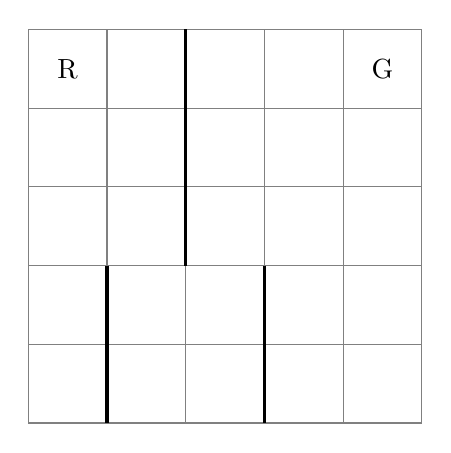
\begin{tikzpicture}
            \draw[step=1cm,color=gray] (0,0) grid (5,5);
            \node at (0.5,4.5) {R};
            \node at (4.5,4.5) {G};
            \draw[very thick] (2,5) -- (2,3);
            \draw[very thick] (1,2) -- (1,0);
            \draw[very thick] (3,2) -- (3,0);
            \draw[very thick] (2,3) -- (2,2);
        \end{tikzpicture}}}
    \caption{Original and modified 'Taxi' environments. The thick black lines represent the walls, while the dotted lines represent the "traps".}
    \label{fig:taxi}
\end{figure}

\section{Implementation of the DQN agents}

Some initial testing of the state decomposition method has been conducted in the "Taxi-v3" environment. Here, the state-decomposition method modified to skip the second stage of joining the networks together showed equivalent performance as a single DQN agent. The equivalence is to be expected since in this environment the sub-problems are completely independent and it does not prove anything about the algorithm in general. One issue of the testing conducted until now is the format in which the states were fed into the Neural Networks. The OpenAI Gym library represents discrete states and actions as single integers. Such a representation is optimal when using tabular Q-learning, as the representations of states and actions simply act as indexes and don't need to be meaningful. However, when using a Q-function approximator, such a meaningless representation impedes the generalisation properties in unseen states that make DQN so useful. Representing the states as one-hot encoded versions of the original integer has also been tested. Though this could allow using shallower neural networks as the decoding of the states is simpler, this is still not a meaningful representation of the states. The current state of the code of the state-decomposition agent is given in the Appendix. To take full advantage of the generalisation to unseen states property of DQN, the format in which states are input to the agents will be modified to be a meaningful representation. This could be in a vector format, where each element of the vector represents a different aspect, such as position, destination, etc.

\section{Timeline}

Figure-\ref{fig:gantt} shows the timeline of my previous and future planned work for this project. The work in April and May could vary considerably depending on the success of the state-decomposition method in testing. If the state-decomposition is tested and shows good performance, it will be possible to focus on some of the extensions described in the next section. In the opposite case, this time will be dedicated to fixing possible problems.

\begin{figure}[H]
    \centering
    \noindent\resizebox{\textwidth}{!}{
    \begin{tikzpicture}[]
    \begin{ganttchart}[
    hgrid,
    vgrid,
    x unit=0.5mm,
    progress=today,
    progress label text=\relax,
    today=2021-02-01,
    time slot format=isodate,
    ]
    {2020-10-01}{2021-06-25}{month=name}
    \gantttitlecalendar{year, month=shortname} \\
    
    \ganttbar{Learning about RL}{2020-10-20}{2020-11-5}\\
    \ganttbar{Literature Review}{2020-10-30}{2021-01-10}\\
    \ganttbar{Try basic RL algorithms in TF on AWS}{2020-11-15}{2020-12-15}\\
    \ganttbar{Code state-decomp. agent with Keras on Colab}{2020-12-12}{2021-01-11}\\
    \ganttbar{Interim Report write-up}{2021-01-05}{2021-02-01}\\
    \ganttbar{Code new TaxiTraps environment}{2021-02-01}{2021-02-14}\\
    \ganttbar{Conduct testing on TaxiTraps}{2021-02-10}{2021-02-30}\\
    \ganttbar{Test approximating transition matrix from sampling}{2021-02-30}{2021-03-15}\\
    \ganttbar{Find more complex environment for testing}{2021-03-05}{2021-03-20}\\
    \ganttbar{Testing in more complex environment}{2021-03-20}{2021-04-05}\\
    \ganttbar{Testing of benchmarks}{2021-04-05}{2021-04-15}\\
    \ganttbar{Work on extensions/problems}{2021-04-15}{2021-05-31}\\
    \ganttbar{Draft report write-up}{2021-05-10}{2021-05-31}\\
    \ganttbar{Final report}{2021-06-01}{2021-06-16}\\
    \ganttbar{Final presentation}{2021-06-17}{2021-06-22}
    
    \ganttlink{elem0}{elem2}
    \ganttlink{elem3}{elem5}
    \ganttlink{elem5}{elem6}
    \ganttlink{elem6}{elem8}
    \ganttlink{elem8}{elem9}
    
    \end{ganttchart}
    \end{tikzpicture}}
    \caption{Gantt chart of previous and future work plan.}
    \label{fig:gantt}
\end{figure}



\section{Extensions}

\paragraph{Compression and embeddings of states} The state-decomposition algorithm divides the original state-space of the system into smaller groups of states. It can be supposed that the variance of the states within these sub-spaces is smaller than in the original state space. Thus, the states that are input in the sub-spaces' agents could be successfully compressed into a more compact representation which could positively affect the performance of the algorithm. More generally, it could be beneficial to learn custom embeddings for the states of each sub-space, having the aim of better generalisation rather than state-space reduction.

\paragraph{Applying state-decomposition to continuous state-spaces} The state-decomposition method is only applicable to discrete state spaces. A possible extension would investigate methods to decompose continuous state-spaces. A state-transition matrix could be obtained by discretising the states and the state-space would be decomposed accordingly, while the agents could still be fed the original continuous states as input.

\paragraph{Applying threshold to transitions between whole sub-spaces} The original state-decomposition method in this project consists of temporarily ignoring improbable state transitions by applying a threshold to the state-transition matrix. There are scenarios in which groups of states are connected by state-transitions that have a high probability but it would still be useful to consider them as separate sub-spaces. Consider for example Figure-\ref{fig:connected-states}, where an MDP is composed of nearly independent sub-spaces that are only connected by the blue transitions. In such a scenario it could be useful to determine the sub-spaces by limiting the number of possible non-zero transition probabilities between any two sub-spaces rather than applying a probability threshold to every single transition. Alternatively, we could apply a threshold to transition probabilities between sub-spaces instead of single states.

\paragraph{Offline training} The samples obtained from the pre-training interaction required to obtain the state-transition matrix could be saved and later added to the experience replay memories of the DQN agents. Offline pre-training could also be conducted using these samples as this could improve sample efficiency. Similarly, transition samples between different sub-spaces are not used in the first stage of training. These could be used to conduct offline pre-training of the merged network.

%\paragraph{Sharing information between sub-agents}

\begin{figure}[H]
    \centering
    \resizebox{0.5\linewidth}{!}{
    \begin{tikzpicture}[]

        % Setup the style for the states
        \tikzset{node style/.style={state, 
                                    minimum width=1cm,
                                    line width=0.5mm,
                                    fill=gray!20!white}}

        % Draw the states
        \node[node style] at (0, 0) (0) {0};
        \node[node style] at (3, 0) (1) {1};
        \node[node style] at (0, -3) (2) {2};
        \node[node style] at (3, -3) (3) {3};
        
        \node[node style] at (6, 0) (4) {4};
        \node[node style] at (9, 0) (5) {5};
        \node[node style] at (6, -3) (6) {6};
        \node[node style] at (9, -3) (7) {7};
        
        \node[node style] at (0, -6) (8) {8};
        \node[node style] at (3, -6) (9) {9};
        \node[node style] at (0, -9) (10) {10};
        \node[node style] at (3, -9) (11) {11};
        
        \node[node style] at (6, -6) (12) {12};
        \node[node style] at (9, -6) (13) {13};
        \node[node style] at (6, -9) (14) {14};
        \node[node style] at (9, -9) (15) {15};

        % Connect the states with arrows
        \draw[every loop,
                auto=right,
                line width=0.5mm,
                >=latex,
                draw=orange,
                fill=orange]
            (2)     edge[bend right=20]            node {} (0)
            (2)     edge[bend right=20, auto=left] node {} (1)
            (2)     edge[bend right=20, auto=left] node {} (3)
            (2)     edge[loop left=20, auto=left] node {} (2)
            (1)     edge[bend right=20]            node {} (2)
            (1)     edge[bend right=20, auto=left] node {} (0)
            (1)     edge[loop right=20, auto=left] node {} (1)
            (1)     edge[bend right=20, auto=left] node {} (3)
            (0) edge[bend right=20]            node {} (1)
            (0)     edge[bend right=20, auto=left] node {} (3)
            (0) edge[bend right=20, auto=left] node {} (2)
            (0)     edge[loop left=20, auto=left] node {} (0)
            (3) edge[bend right=20]            node {} (1)
            (3)     edge[bend right=20, auto=left] node {} (0)
            (3) edge[bend right=20, auto=left] node {} (2)
            (3)     edge[loop right=20, auto=left] node {} (3)
            
            (6)     edge[bend right=20]            node {} (4)
            (6)     edge[bend right=20, auto=left] node {} (5)
            (6)     edge[bend right=20, auto=left] node {} (7)
            (6)     edge[loop left=20, auto=left] node {}  (6)
            (5)     edge[bend right=20]            node {} (6)
            (5)     edge[bend right=20, auto=left] node {} (4)
            (5)     edge[loop right=20, auto=left] node {} (5)
            (5)     edge[bend right=20, auto=left] node {} (7)
            (4) edge[bend right=20]            node {}     (5)
            (4)     edge[bend right=20, auto=left] node {} (7)
            (4) edge[bend right=20, auto=left] node {}     (6)
            (4)     edge[loop left=20, auto=left] node {}  (4)
            (7) edge[bend right=20]            node {}     (5)
            (7)     edge[bend right=20, auto=left] node {} (4)
            (7) edge[bend right=20, auto=left] node {}     (6)
            (7)     edge[loop right=20, auto=left] node {} (7)
            
            (10)     edge[bend right=20]            node {} (8)
            (10)     edge[bend right=20, auto=left] node {} (9)
            (10)     edge[bend right=20, auto=left] node {} (11)
            (10)     edge[loop left=20, auto=left] node {} (10)
            (9)     edge[bend right=20]            node {} (10)
            (9)     edge[bend right=20, auto=left] node {} (8)
            (9)     edge[loop right=20, auto=left] node {} (9)
            (9)     edge[bend right=20, auto=left] node {} (11)
            (8) edge[bend right=20]            node {}     (9)
            (8)     edge[bend right=20, auto=left] node {} (11)
            (8) edge[bend right=20, auto=left] node {}     (10)
            (8)     edge[loop left=20, auto=left] node {}  (8)
            (11) edge[bend right=20]            node {}     (9)
            (11)     edge[bend right=20, auto=left] node {} (8)
            (11) edge[bend right=20, auto=left] node {}     (10)
            (11)     edge[loop right=20, auto=left] node {} (11)
            
            (14)     edge[bend right=20]            node {} (12)
            (14)     edge[bend right=20, auto=left] node {} (13)
            (14)     edge[bend right=20, auto=left] node {} (15)
            (14)     edge[loop left=20, auto=left] node {}  (14)
            (13)     edge[bend right=20]            node {} (14)
            (13)     edge[bend right=20, auto=left] node {} (12)
            (13)     edge[loop right=20, auto=left] node {} (13)
            (13)     edge[bend right=20, auto=left] node {} (15)
            (12) edge[bend right=20]            node {}     (13)
            (12)     edge[bend right=20, auto=left] node {} (15)
            (12) edge[bend right=20, auto=left] node {}     (14)
            (12)     edge[loop left=20, auto=left] node {}  (12)
            (15) edge[bend right=20]            node {}     (13)
            (15)     edge[bend right=20, auto=left] node {} (12)
            (15) edge[bend right=20, auto=left] node {}     (14)
            (15)     edge[loop right=20, auto=left] node {} (15)
            (3) edge[bend right=20, draw=blue, fill=blue]            node {}     (6)
            (6)     edge[bend right=20, auto=left, draw=blue, fill=blue] node {} (12)
            (12) edge[bend right=20, auto=left, draw=blue, fill=blue] node {}     (9)
            (9)     edge[bend right=20, auto=left, draw=blue, fill=blue] node {} (3);
    \end{tikzpicture}}
    \caption{MDP composed of smaller subspaces of states connected by few but probable transitions.}
    \label{fig:connected-states}
\end{figure}


\paragraph{Using state-decomposition for automatic sub-goal discovery} The idea of state-decomposition, especially when implemented by considering transitions between whole sub-spaces could be applied to the automatic discovery of sub-goals in hierarchical reinforcement learning. A similar idea has been adopted by \cite{simsek_identifying_2005} and \cite{menache_q-cutdynamic_2002}, in which the graph of the MDP is divided into sub-spaces by cutting through the least possible number of state-transitions. The intuition is that sub-goals, such as driving towards the passenger in "Taxi-v3" or driving to the destination after picking it up, are often connected by bottleneck states, such as states 3, 6, 9 and 12 in Figure-\ref{fig:connected-states}.


%\paragraph{No NN version} For the ersion without neural networks, the final neural netowrk could be attached earlier than achiving convergence if we still allow to update the intermediate q-values during training

%if I do without NN I don't think it's really state decomposition. It's more like I initially do q-learning in a simple environment that disregards interactions between subsystems and then I append a NN at the end to take into account these interatctions, Seems like a very weird thing to do doesn't it

%\paragraph{aybe prove some mathematical bounds}

%\paragraph{Possible expansion of looking at how policy affects the decomposition}

%%%%%%%%%%%%%%%%%%%%%%%%%%%%%%%%%%%%
\chapter{Evaluation Plan}

%Differently from many other projects, this project does not have as a goal a certain application for which different techniques can be used. Thus the eventual success of the project can't be evaluated by the success of the application. In this project, we are developing the technique itself, which could then be applied in different contexts. Since the project consists of the development of a new algorithm, there is no certainty that the algorithm would achieve good performance. Thus, the project can be considered successful even if the state-decomposition algorithm does not show improved performance.

The main objective of this project is to evaluate the performance of the proposed state-decomposition algorithm. To do so, the algorithm will be tested in different varieties in the TaxiTraps environment described in Section-\ref{sec:TaxiTraps}. The possible varieties are:

\begin{itemize}
    \item In the original state-decomposition algorithm it is assumed that the NNs of the sub-spaces' agents keep training after they are joined together in the second stage of the training as they are part of the bigger newly formed neural network of the global agent. Alternatively, we could freeze the weights of the sub-spaces' NNs (trained in the 1st stage) during the second stage of training. 
    
    \item Once the NNs are joined in the 2nd stage, the training could be done using all transitions, only those that start and end in different sub-space\footnote{To take into account the transitions between different sub-spaces.} or start with only transitions between different sub-spaces\footnote{At this stage of training we have many of these transitions that were saved but ignored in the first stage of training.} and then as the global agent experiences more transitions use all possible transitions.
    
    \item The time at which the agents of the sub-spaces should be joined together to form the global agent is not defined. Different strategies can be compared, such as waiting for the sub-agents' action-values to converge or defining different minimum rates of change of the average episode rewards going below which would start the second stage of training.
\end{itemize}

\paragraph{}
The main aspect of these algorithms that will be evaluated is the sample efficiency, which is how efficiently the algorithm uses the samples that it experiences to learn a policy. This affects how quickly the algorithm can learn an optimal policy and it can be measured by plotting the total reward per episode vs the number of training steps. It is also important to consider the fact that the learning process is stochastic and the performance varies between trials, hence we normally express the reward per episode using a confidence bound.

\begin{figure}[H]
%\begin{wrapfigure}{r}{0.5\linewidth}
    \centering
    \includegraphics[width=0.5\linewidth]{figures/exampleOfGraph.PNG}
    \caption{Example of reward per episode vs number of training steps. Note the confidence bands to express the uncertainty in the results. Figure taken from \cite{stateActionEmbeddings}}
    \label{fig:my_label}
%\end{wrapfigure}
\end{figure}

\paragraph{}
All these variations of the state-decomposition method will be compared with a standard DQN agent. There are many scenarios where the system is known to be formed by almost independent sub-systems corresponding to almost independent sub-problems. In such a scenario, the states could be grouped into separate sub-spaces without even estimating the state-transition matrix by just leveraging the knowledge of the characteristics of the system. Thus, we shall compare the performance of the state-decomposition method when the state-transition matrix is given (or sub-spaces can be guessed) at the start and when it has to be estimated from samples. In the latter case, we can estimate the model of the environment is we also consider the rewards of the samples. Thus we shall also compare the performance of the state-decomposition algorithm with a method that simply approximates the model of the environment from samples and then finds the optimal policy using planning algorithms. 

THINGS TO CARE ABOUT:

When I use the deltaswitch, how the weights updated for NN0 when NN1 is active and vice-versa.
https://www.gatsby.ucl.ac.uk/~dayan/papers/cjch.pdf
https://arxiv.org/pdf/1901.00137.pdf
relationship with drpout
gains might be due to effects of double q-learning rather than decomposition
resource allocation / job allocation 
alibaba datasetF


%%%%%%%%%%%%%%%%%%%%%%%%%%%%%%%%%%%%
\chapter{Ethical, Legal, and Safety Plan}

Following a brief consultation with my project supervisor, I can state that this project does not involve any kind of ethical, legal, or safety issues. 

\paragraph{Ethical Issues} The project does not involve experimentation with humans or animals and it is not going to cause any physical or psychological harm to any participants. 

\paragraph{Legal Issues} The project doesn't involve the participation of people in surveys or any kind of collection of sensitive data, meaning that privacy is not an issue. This is an open research project and it is not affected by any copyrights or confidentiality agreements. This work is also not affected by any existing patents. 
\paragraph{Safety Issues} The project work is extremely unlikely to cause any physical harm as it doesn't involve the operation of dangerous equipment involving any high voltages, chemicals, flammable materials, biological hazards, etc.


\singlespacing

%% bibliography
\bibliographystyle{ieeetr}
\bibliography{bibliography/bibliography,bibliography/zotero}

%%%%%%%%%%%%%%%%%%%%%%%%%%%%%%%%%%%%
\appendix
\chapter{Code}
\label{appendix}

\lstset{language=Python,
  basicstyle=\small,breaklines=true}

\paragraph{Function for State Decomposition}
\begin{lstlisting}[caption={Function which is given the state-transition matrix in input and combines the thresholding of its values with the decomposition into separate MDPs, returning \texttt{d} which is a list indicating which sub-space each state belongs to (as an index) and \texttt{groups} which is a list of lists containing the states of each sub-space.}, captionpos=b]
def stateDecomposition(st_table, thr):
  def joinGroups(i, j, d, groups):
    M = max(d[i], d[j])
    m = min(d[i], d[j])
    if d[i] != d[j]:
      groups[m] += groups[M]
      del groups[M]
      for ind, el in enumerate(d):
        if el > M: d[ind] -= 1
        if el == M: d[ind] = m

  n_states = st_table.shape[0]
  d = [i for i in range(n_states)]
  groups = [[i] for i in range(n_states)]

  #iterate through all the entries
  for i, j in np.ndindex(st_table.shape):
    if st_table[i][j] > thr: joinGroups(i, j, d, groups)
          
  return d, groups
\end{lstlisting}

\paragraph{Function for State Decomposition given target number of subspaces}
\begin{lstlisting}[caption={Function that given the state-transition and a target number of subspaces performs the state-decomposition with different thresholds in order to obtain the correct number of subspaces.}, captionpos=b]
def stateDecompositionWithNGroups(st_table, target_n_groups):
  limitIterations = 50 # number of iterations after which the algorithm stops 
  firstChangeFactor = 10.0 # factor by which the threshold is multiplied/divided after first iteration
  thr = 1.0 # initial threshold

  lowerBound = None
  upperBound = None

  for i in range(limitIterations):
    if lowerBound == None and upperBound != None: thr = upperBound / firstChangeFactor
    if lowerBound != None and upperBound == None: thr = lowerBound * firstChangeFactor
    if lowerBound != None and upperBound != None: thr = (upperBound + lowerBound) / 2.0

    stateGroups = stateDecomposition(st_table, thr)
    n_groups = len(stateGroups[1])
    if n_groups == target_n_groups: 
      print("Target number achieved")
      break
    if n_groups < target_n_groups: lowerBound = thr
    if n_groups > target_n_groups: upperBound = thr
    print(thr)

  return stateGroups, thr
\end{lstlisting}

\paragraph{Class for State Decomposition DQN Agent}
\begin{lstlisting}[caption={Current version of my state-decomposition agent. In this version the states are fed in the neural networks as one-hot-encoded integers.}, captionpos=b]
class StateDecompositionDQNAgent:
  def __init__(self, state_size, action_size, subnetIndexes, subnets):
    self.state_size = state_size
    self.action_size = action_size
    self.gamma = 0.95    # discount rate
    self.epsilon = 1.0  # exploration rate
    self.epsilon_min = 0.01
    self.epsilon_decay = 0.999
    self.learning_rate = 0.001
    self.subnets = subnets
    self.n_subnets = len(stateGroups[1])
    self.subnetIndex = self._subnetIndex_init(subnetIndexes)
    self.memory = [deque(maxlen=50000) for i in range(len(self.subnets)+1)]
    self.models = self._build_models()

  def _subnetIndex_init(self, subnetIndexes):
    ind0s = subnetIndexes
    ind1s = [np.where(self.subnets[ind0s[i]] == i)[0][0] for i in range(self.state_size)]
    return list(zip(ind0s, ind1s))

  def _number_to_one_hot(self, n_classes, x):
    one_hot_vect = np.eye(n_classes)[x]
    reshaped = np.reshape(one_hot_vect, (1, n_classes))
    return reshaped

  def _one_hot_subnet(self, state):
    ind0, ind1 = self.subnetIndex[state]
    n_classes = self.subnets[ind0].shape[0]
    return self._number_to_one_hot(n_classes, ind1)

  def _all_zeros(self, subnet):
    l = len(subnet)
    return np.zeros((1,l))
    
  def _one_hot_joined(self, state):
    ind0, _ = self.subnetIndex[state]
    one_hot_inputs = []
    for i, subnet in enumerate(self.subnets):
      if i == ind0:
        one_hot_inputs.append(self._one_hot_subnet(state))
      else:
        one_hot_inputs.append(self._all_zeros(subnet))
    return np.concatenate(one_hot_inputs, axis=1)
    
  def _build_subnet_model(self, subnet):
    subLen = len(subnet)
    inputs = Input(shape=(subLen,), name="input{}".format(subLen))
    x = Dense(50, activation='relu', name="subnet{}_dense_0".format(subLen))(inputs)
    x = Dense(50, activation='relu', name="subnet{}_dense_1".format(subLen))(x)
    x = Dense(50, activation='relu', name="subnet{}_dense_2".format(subLen))(x)
    out = Dense(self.action_size, activation='linear', name="subnet{}_dense_3".format(subLen))(x)
    model = Model(inputs=inputs, outputs=out, name="model{}".format(subLen))
    model.compile(loss='mse',
                  optimizer=Adam(lr=self.learning_rate))
    return model
    
  def _build_models(self):
    return [self._build_subnet_model(s) for s in self.subnets]

  def join_models(self):
    def _joined_subnets(input):
      ind = 0
      outputs = []
      for i, subnet in enumerate(self.subnets):
        input_subnet = Lambda(lambda x: x[:,i:i+len(subnet)], name="lambda_{}".format(i))(input)
        return Lambda(lambda x: x[:,i:i+len(subnet)], name="lambda_{}".format(i))(input)
        outputs.append(self.models[i](input_subnet))
        i += len(subnet)
      return Concatenate(name="concatenate_int_outputs")(outputs)

    def _top_network(input):
      n_inputs = self.action_size * self.n_subnets
      x = Dense(24, activation='relu', input_shape=(None,n_inputs,), name="top_dense_0")(input)
      x = Dense(48, activation='relu', name="top_dense_1")(x)
      x = Dense(48, activation='relu', name="top_dense_2")(x)
      x = Dense(self.action_size, activation='linear', name="top_dense_3")(x)
      return x

    input = Input(shape=(self.state_size,), name="intermediate_input")
    int_outputs = _joined_subnets(input)
    output = _top_network(int_outputs)
    model = Model(inputs=input, outputs=output, name="joined_model")
    model.compile(loss='mse',
                  optimizer=Adam(lr=self.learning_rate)) #maybe should have separate lr for the top model
    self.models.append(model)

  def remember_subnet(self, state, action, reward, next_state, done):
    ind0, _ = self.subnetIndex[state]
    next_ind0, _ = self.subnetIndex[next_state]
    if ind0 == next_ind0:
      self.memory[ind0].append((state, action, reward, next_state, done))
      return ind0
    self.memory[self.n_subnets].append((state, action, reward, next_state, done))
    return -1

  def remember_joined(self, state, action, reward, next_state, done):
    self.memory[self.n_subnets].append((state, action, reward, next_state, done))

  def act_subnet(self, state):# We implement the epsilon-greedy policy
    if np.random.rand() > self.epsilon:
      one_hot_state = self._one_hot_subnet(state)
      model = self.models[self.subnetIndex[state][0]]
      act_values = model.predict(one_hot_state)
      return np.argmax(act_values[0]) # returns action
    return random.randrange(self.action_size)
    
  def exploit(self, state): # When we test the agent we dont want it to explore anymore, but to exploit what it has learnt
    act_values = self.models[self.n_subnets].predict(self._one_hot_joined(state))
    return np.argmax(act_values[0]) 

  def act_joined(self, state):# We implement the epsilon-greedy policy
    if np.random.rand() > self.epsilon:
      return self.exploit(state) # returns action
    return random.randrange(self.action_size)


  def replay(self, subnet_ind, batch_size, joined):
    if joined:
      index = self.n_subnets
    else: 
      index = subnet_ind
    
    minibatch = random.sample(self.memory[index], batch_size)

    b = False
    for el in minibatch:
      if self.subnetIndex[el[0]][0] != subnet_ind or self.subnetIndex[el[3]][0] != subnet_ind:
        return True
    if b: print("WRONG")

    action_b = np.squeeze(np.array(list(map(lambda x: x[1], minibatch))))
    reward_b = np.squeeze(np.array(list(map(lambda x: x[2], minibatch))))
    done_b = np.squeeze(np.array(list(map(lambda x: x[4], minibatch))))

    ### Q-learning
    if joined:
      state_b_one_hot = np.squeeze(np.array(list(map(lambda x: self._one_hot_joined(x[0]), minibatch))))
      next_state_b_one_hot = np.squeeze(np.array(list(map(lambda x: self._one_hot_joined(x[3]), minibatch))))
    else: 
      state_b_one_hot = np.squeeze(np.array(list(map(lambda x: self._one_hot_subnet(x[0]), minibatch))))
      next_state_b_one_hot = np.squeeze(np.array(list(map(lambda x: self._one_hot_subnet(x[3]), minibatch))))

    pred = self.models[index].predict(next_state_b_one_hot)
    target = (reward_b + self.gamma * np.amax(pred, 1))
    target[done_b==1] = reward_b[done_b==1]
    target_f = self.models[index].predict(state_b_one_hot)

    for k in range(target_f.shape[0]):
      target_f[k][action_b[k]] = target[k]
    self.models[index].train_on_batch(state_b_one_hot, target_f)
    if self.epsilon > self.epsilon_min:
        self.epsilon *= self.epsilon_decay

  def load(self, name):
    self.model.load_weights(name)
  def save(self, name):
    self.model.save_weights(name)
\end{lstlisting}

\end{document}
